\documentclass[11pt,dvipdfmx,a4paper]{jsarticle}

\usepackage{amsmath,amssymb}
\usepackage{bm}
\usepackage[dvipdfmx]{graphicx}
\usepackage{physics} % http://mirrors.ibiblio.org/CTAN/macros/latex/contrib/physics/physics.pdf
\usepackage{siunitx} %SI単位を楽に出力
\usepackage{mathtools} %環境の追加
% \usepackage{circuitikz} %電気回路をtex中で書く
% \usepackage{caption} %番号なしキャプションを書く
% \usepackage{cancel} %式中に斜線を入れる
% \usepackage{tensor} %テンソルの添え字を書く
% \usepackage{tikz} %図を書く
% \usepackage{ascmac} %四角い枠の中に文章を書く
% \usepackage{float} %figureで[hbp]オプションを使う
% \usepackage{hyperref}  \usepackage{pxjahyper} %ハイパーリンクをつかう
% \usepackage{tablefootnote} %表中に注釈をいれる
% \usepackage[thicklines]{cancel} %数式中の取り消し線
\usepackage[version=4]{mhchem} %化学式の入力
\usepackage{pdfpages}
\usepackage{wrapfig} %文章の回り込み
\usepackage[subrefformat=parens]{subcaption} %(a)図のようにすることができるやつ
\usepackage{here}
\usepackage{mathrsfs} % フォントの追加
\usepackage{url} % url を入れる
\usepackage[margin=15mm]{geometry} %余白の削除

\graphicspath{{./image/}}

\begin{document}

%出力したpdfを表紙にするとき
% \includepdf[pages=1,noautoscale=false]{cover.pdf}
% \newpage

%texで表紙を書くとき
\quad\\[35mm]
\centerline{\Huge{\textsf{第 5 回}}}
\quad\\[5mm]
\centerline{\Huge{\textsf{応 用 物 理 学 実 験}}}
\quad\\[5mm]
\begin{table}[h]
	\centering
	\begin{tabular}{| c | c |}
		\hline
		\Huge\textsf{{題目}} & \Huge{\textsf{半導体}} \rule[-5mm]{0mm}{15mm} \\
		\hline
	\end{tabular}
\end{table}
\quad\\[10mm]
\begin{table}[h]
	\centering
	\begin{tabular}{l l}
		\hline
		\LARGE{\textsf{氏\qquad 名}} & \LARGE{\textsf{: 西原 翔}} \rule[0mm]{0mm}{6mm} \\
		\hline
		\LARGE{\textsf{学  籍  番  号}} & \LARGE{\textsf{: 1522068}} \rule[0mm]{0mm}{6mm} \\
		\LARGE{\textsf{学部学科学年}} & \LARGE{\textsf{: 理学部第一部応用物理学科3年}}\\
		\hline
	\end{tabular}
\end{table}
\quad\\[10mm]
\centerline{\LARGE{\textsf{共同実験者:1522064 中井空弥}}}\\[2mm]
\quad\\[10mm]
\centerline{\LARGE{\textsf{提出年月日:2024年07月18日}}}\\[2mm]
\centerline{\LARGE{\textsf{実験実施日:2024年06月28日}}}\\[2mm]
\centerline{\LARGE{\textsf{\qquad\qquad\quad\;2024年07月05日}}}
\quad\\[10mm]
\centerline{\LARGE{\textsf{東 京 理 科 大 学 理 学 部 第 1 部}}}\\[2mm]
\centerline{\LARGE{\textsf{応 用 物 理 学 教 室}}}

\thispagestyle{empty}
\clearpage
\addtocounter{page}{-1}
\newpage

% \twocolumn
\section{目的}

\section{原理}
\subsection{素励起と準粒子}
結晶中の電子の振舞いについて考える。
1つの孤立している原子を考える。
電子はその原子核に束縛され、離散的なエネルギー準位をとるようになる。
その原子が2つ近づくと、相互作用により元のエネルギー準位が分裂して2つのエネルギー準位をとるようになる。
固体中であるためこのような相互作用が多数あるため、分裂したエネルギー準位はほとんど連続的なものとみなすことができる。
これがバンドである。

そうしたバンドの準位に電子は低いエネルギーから入っていく。
その際、
パウリの排他原理によりエネルギーの低い状態となっている電子は外乱により別の状態に遷移しようとしても、
すでにほかの電子がその状態を占めているため、状態を変えることが禁じられる。
一方、エネルギーの最も高い状態付近(フェルミ面)の電子は外乱により別の状態に遷移する際に、
フェルミ面より高い準位や、他の電子がすでに励起して空になったエネルギー準位遷移することができる。

これより、結晶に外乱をいれたときに応答に関わってくるのはフェルミ面付近だけ考えばよくなる。
これはもっと言うと、フェルミ面内部にある電子は系の応答に関わらないため無視をして、
励起によりフェルミ面の外に出た電子や空になった準位だけを考えることができる。
つまり、結晶の現象はフェルミ面を新たな真空として、その真空で対生成・対消滅する電子と正の電荷をもった孔(正孔)によるものだということができる。
このような描像を素励起といい、これらにより生成・消滅する粒子を準粒子というように呼ばれる。

\begin{wrapfigure}{r}[0pt]{0.4\columnwidth}
	\centering
	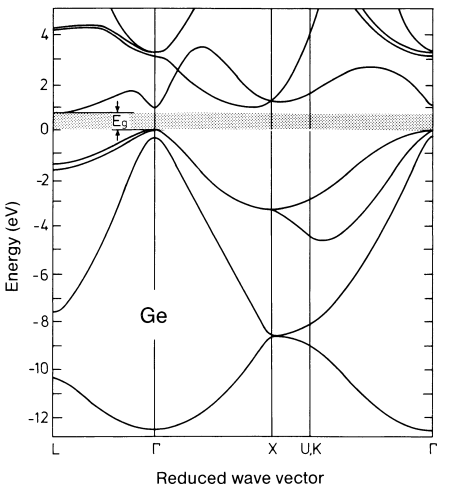
\includegraphics[width=0.4\columnwidth]{graph/graph01.png}
	\caption{Ge のバンド図\cite{ibach-luth}}
	\label{graph:01}
\end{wrapfigure}
この描像では結晶を構成する原子核の周期的ポテンシャルというのは、
準粒子の質量に取り込まれる。
このように周期的ポテンシャルを取り込んだ質量を有効質量と呼ぶ。
そのため準粒子としての電子は、
同じ電子という名前が付いているが実態としては真空中の電子とは異なり、
一定の質量をもたないような別の粒子になっている。
正孔というのも名前に孔というようにあるが、しっかりと(有効)質量をもった粒子とみなす。

有効質量は定量的にはバンドの曲率として定義される。
つまり
\begin{equation}
	\frac{1}{m_{ij}} = \pdv[2]{E(\vb*{k})}{k_i}{k_j}
\end{equation}
として定義される。
波数空間が等方的であるときには有効質量はテンソル量ではないスカラー量
\begin{equation}
	\frac{1}{m} = \pdv[2]{E(\vb*{k})}{k}
\end{equation}
となる。
有効質量によって周期的ポテンシャルというのは準粒子の運動方程式に現れなくなり、
自由粒子と同じ運動方程式となる。なので準粒子は固体内部で理想気体のように振舞う。

実際の Ge のバンド図(図\ref{graph:01})との対応を見てみる。
フェルミ面がバンドギャップ\(E_g\)の間を通っている結晶は半導体と呼ばれる。
実際に電子と正孔の対生成・対消滅する場所としては Reduced wave vector が \(\Gamma\)
つまり波数ベクトルが\(\vb*{k}=(0,\,0,\,0)\)の地点にあるエネルギーギャップ付近である。
上下に放物線があり、上にある放物線上に準粒子としての電子が現れ、下にある放物線上に正孔が現れる。
このとき正孔は真空より低い負のエネルギーを持っているように見えるが、
そのようにとらえるのではなく符号を取り直して正のエネルギーを持つものと考える。
\footnote{Dirac が考えた Dirac の海による陽電子の説明と似ている。
歴史的には Peierls が1929年に電子と正孔を用いて Holl 効果を説明してから Dirac の海の話が1930年に出たようである。
Dirac の海による陽電子の予言の偉いところは Dirac の海のような描像を思いつた点ではなく、
電子と正孔の生成というのがフェルミ面という"真空"で粒子が対生成・対消滅していて、
真空でもこれと同様なことを思いついた点であるのだろう。ただこの話の証拠はないため私の妄想ではある。}
フェルミ面を真空としているので、フェルミ面のエネルギーを 0 とすると\footnote{図\ref{graph:01}の縦軸のエネルギーの基準点とは違う基準}、
この放物線はそれぞれ、
\begin{align}
	E(k) &= \frac{E_g}{2} + \frac{\hbar^2k2}{2m_e^*}\\
	E(k) &= \frac{E_g}{2} - \frac{\hbar^2k2}{2m_p^*}
\end{align}
となる。ここで\(m_e^*\)を電子の有効質量、\(m_p^*\)を電子の有効質量とした。
また簡単のためフェルミ面はエネルギーギャップのちょうど真ん中にあるものとしている。 % TODO ほんまか?
電子・正孔の分散関係と呼ばれ、分散関係がわかるとエネルギーの幅が\([E,\,E+dE]\)の間にとることのできる状態の数を表す(有効)状態密度\(D(E)dE\)というのも求められる。

エネルギー\(E(k)\)における状態密度は
\begin{align}
	D(E)
	&= 2\times\sum_k \delta(E-E(k)) \notag\\
	&= \frac{2V}{(2\pi^3)}\int d\vb*{k}\, \delta\qty(E-\frac{E_g}{2} - \frac{\hbar^2k^2}{2m^*}) \notag\\
	&= \frac{V}{\pi^2} \int dk\, k^2\times \frac{1}{2}\sqrt{\frac{\hbar^2}{2m^*(E-E_g/2)}}\qty{\delta\qty(k-\sqrt{\frac{2m^*(E-E_g/2)}{\hbar^2}})+\delta\qty(k+\sqrt{\frac{2m^*(E-E_g/2)}{\hbar^2}})} \notag\\
	&= \frac{V}{2\pi^2}\qty(\frac{\hbar^2}{2m^*})^{3/2}\sqrt{E-\frac{E_g}{2}}
\end{align}
として求められる。
また、粒子の分布関数はフェルミ分布関数
\begin{equation}
	f(E) = \frac{1}{1+e^{E/k_BT}}
\end{equation}
で表される。

通常のバンド理論ではフェルミ面より下にあるバンドを価電子帯、上にある伝導帯と呼ばれる。
この呼び方は次のような描像から来ている。
価電子帯と呼ばれるバンドの内部にある電子は、
上の説明からわかるように電気伝導にかかわることはない。
その理由をこの電子は原子核に束縛されて動けない価電子であるからだというように考える。
一方、伝導体と呼ばれるバンドの内部にある電子は素励起による説明における電子になっている。
するとその電子は束縛されていない自由電子で、結晶内を移動していくキャリアとなる。
なので価電子帯や伝導帯のように呼ばれている。
また、正孔にとってはフェルミ面の上側にあるのが価電子帯、下側にあるのが伝導帯となる。

\subsection{半導体への不純物ドーピング}
Ge 半導体に原子番号が隣の元素である \ce{As} か \ce{Ga} の一方を少量だけ混ぜることを考える。
まず初めに \ce{As} を1つだけ加えることを考える。
素励起の描像では \ce{Ge} の結晶だけでは真空であったので、
もともとの \ce{Ge} 結晶からの差分だけが系にあるとみなせる。
\ce{As} の原子核の持つ正電荷は\ce{Ge}の原子核と比較するとだいたい1つ増え、電子が1つ増える。
つまり水素原子と同じ系になっている。
よって新しく追加された電子のシュレーディンガー方程式は
\begin{equation}
	\qty(-\frac{\hbar^2}{2m_e^*}\laplacian - \frac{e^2}{4\pi\varepsilon r})\psi = E \psi
\end{equation}
となる。ここで、\(\varepsilon\)は\ce{Ge}結晶の誘電率である。
\ce{As} に束縛された電子は\ce{Ge}の電子の分散曲線に励起すると自由電子となることから、
エネルギーは伝導体の下端をエネルギーの基準とした
\begin{equation}
	E_n = \frac{E_g}{2} - \frac{m_e^*}{2\hbar^2}\qty(\frac{e^2}{4\pi \varepsilon})^2\frac{1}{n^2}
\end{equation}
というようになる。
追加する不純物は少量であるため、不純物間の間は十分離れてるとみなせる。
なのでこれによるバンド分裂は細くてないものとみなせる。
もともとのエネルギーは eV オーダーの量にたいして、
不純物によってできた新たな準位による束縛エネルギーは meV オーダーである。
これより極端な低温ではないかぎり、熱よって励起をすることができる。
そうして熱励起した電子はキャリアとして半導体内を動くようになる。
なのでキャリアの符号からこれをn型半導体という。

そして\ce{Ga}を加えたときのことを考える。
もともとの \ce{Ge} 結晶からの差分だけが系にあるとみなせる。
\ce{Ga} の原子核の持つ正電荷は\ce{Ge}の原子核と比較するとだいたい1つ減り、電子が1つ減る。
これはつまり、負の電荷をもった原子核の周りに正の電荷をもった正孔があるという水素原子と同じ系となる。
なので\ce{As}のときと同様に考えて
\begin{equation}
	E_n = \frac{E_g}{2} - \frac{m_e^*}{2\hbar^2}\qty(\frac{e^2}{4\pi \varepsilon})^2\frac{1}{n^2}
\end{equation}
というようなエネルギー準位が表れ、
熱により、正孔がキャリアとして励起することができる。
これをp型半導体という。

不純物が入っていない半導体を真性半導体という。
これら3つの簡略化したバンド図は図\ref{fig:01}のようになる。 % TODO もっと説明書く
\begin{figure}[h]
	\centering
	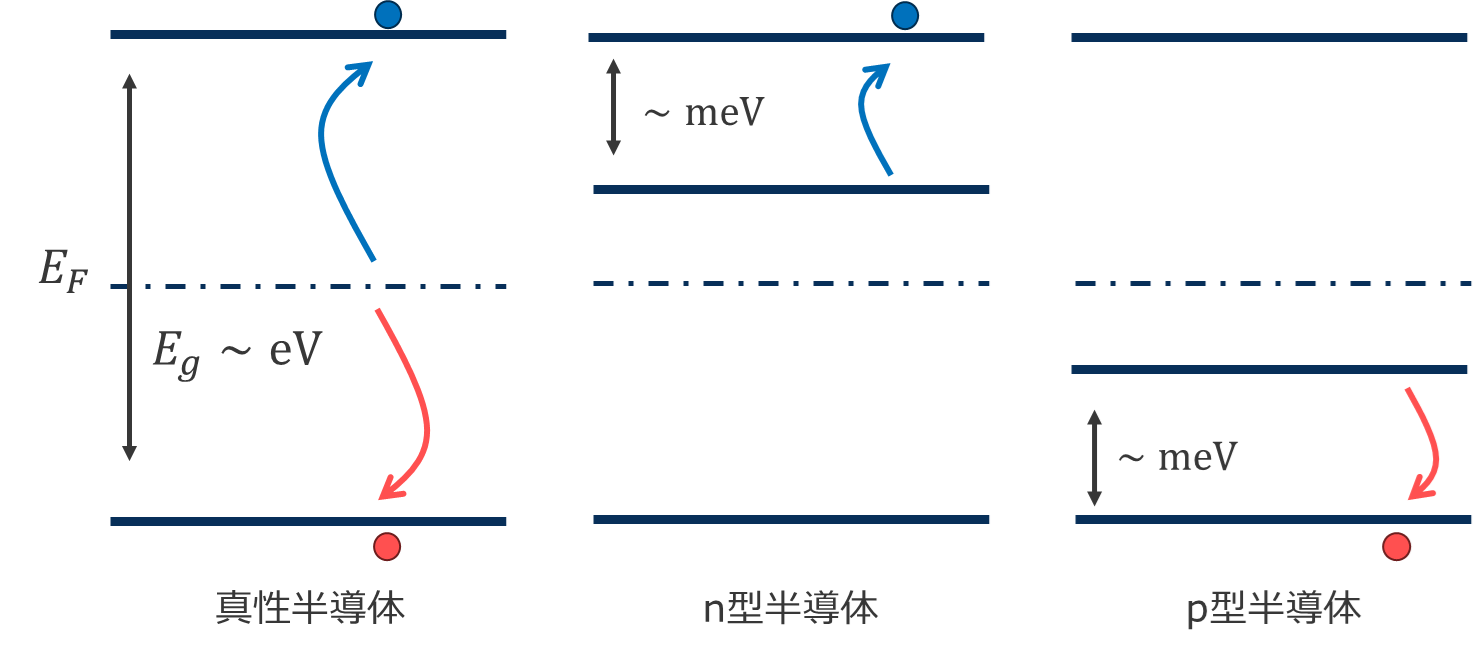
\includegraphics[width=0.65\columnwidth]{fig/fig01.png}
	\caption{不純物を入れたときの簡略化したフェルミ面付近のバンド図}
	\label{fig:01}
\end{figure}


\subsection{ホール効果}

\section{実験}
                                 
\begin{wrapfigure}{r}[0pt]{0.4\columnwidth}
	\centering
	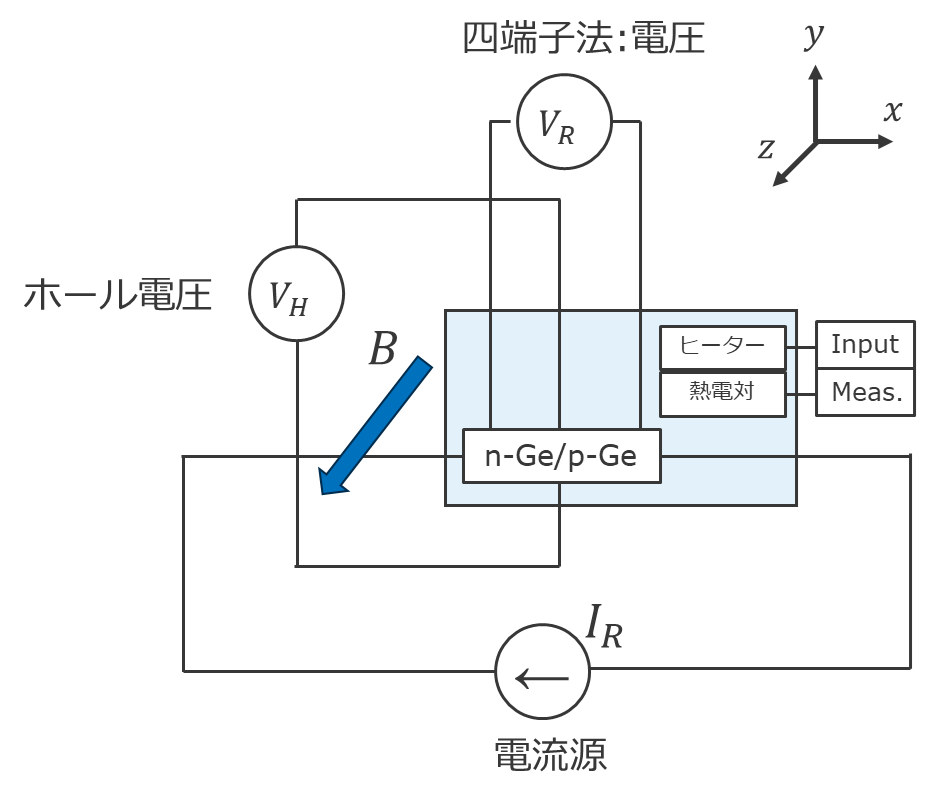
\includegraphics[width=0.4\columnwidth]{fig/fig02.png}
	\caption{測定装置の模式図。ホール電圧を測定するため\(y\)軸方向に端子をつけホール電圧を測定し、
	四端子法で電気伝導度を測定する。過熱をするためのヒーターと温度計として熱電対も装置に組み込まれている。}
	\label{fig:02}
\end{wrapfigure}
\ce{n-Ge}と\ce{p-Ge}の電気伝導にかかわるパラメーターとして電気伝導度と磁場をかけたときのホール係数を試料の温度を変えながら測定した。
測定装置の模式図は図\ref{fig:02}の通りである。
半導体の電気伝導度を測定するには接触抵抗やショットキー障壁といった要素を取り除くため、4端子法で行う。
また、電流を流す方向を\(x\)軸としたときホール電圧を測定する方向を\(y\)軸として、\(z\)軸方向に電磁石によって磁場をかける。
このときホール電圧を測定する端子が\(x\)軸方向へのずれてしまうため、
測定したホール電圧はそのままではずれが生じていることに注意する必要がある。
手順としては、電流を流したときの電磁石の出す磁束密度と電流の関係の校正を行ったのち、
試料のホール電圧の\(x\)軸方向への端子位置のずれを測定するため
-2.4 mA から 2.4 mAの直流電流を流しとゼロ磁場、室温の下で
電気伝導度とホール係数を測定した。
その後、同じ電流の範囲で \(\pm\)50 mT, \(\pm\)100 mT の磁場をかけた下でのホール電圧を測定した。
室温での測定が終わったら、ヒーターを付け試料の温度を上げていく。
1 mA の電流を試料に流しながら、ホール電圧と電気伝導度を測定した。
このとき試料のホール電圧の\(x\)軸方向への端子位置のずれの影響も考慮するため、
ゼロ磁場と 100 mT の磁場をかけたときの両方のホール電圧を測定する必要がある。

\section{結果}

\section{考察}

\section{結論}


\bibliographystyle{junsrt}
\bibliography{reference}
\section*{付録}

\end{document}